\par Les membres du groupe responsables de cette partie étaient Antoine Vallée et Antoine Pietri.

\subsubsection{Textures}
\par Créer un jeu, ce n'est pas seulement le développer, c'est aussi travailler son rendu graphique. Cette tâche n'a pas été une mince affaire. 
\par Le premier travail fut de trouver un fond au jeu, puis des textures. Par la suite, nous devions créer de nombreux missiles. Il a donc fallu faire un travail important sur Photoshop dans le but d'apprendre à s'en servir, et de créer ces missiles.
\par Voici un exemple de rendu en jeu des textures et des missiles:

\begin{center}
	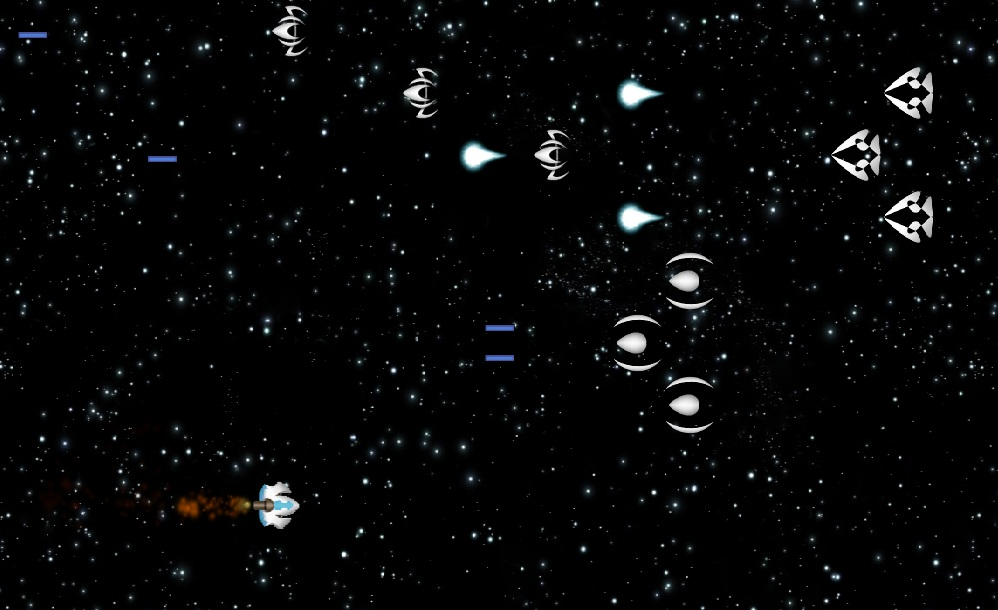
\includegraphics[width=13cm]{images/graphisme1.jpg}
\end{center}

\par De nombreux missiles devaient être dessinés, comme vous pouvez le voir ci dessous:

\begin{center}
	\par 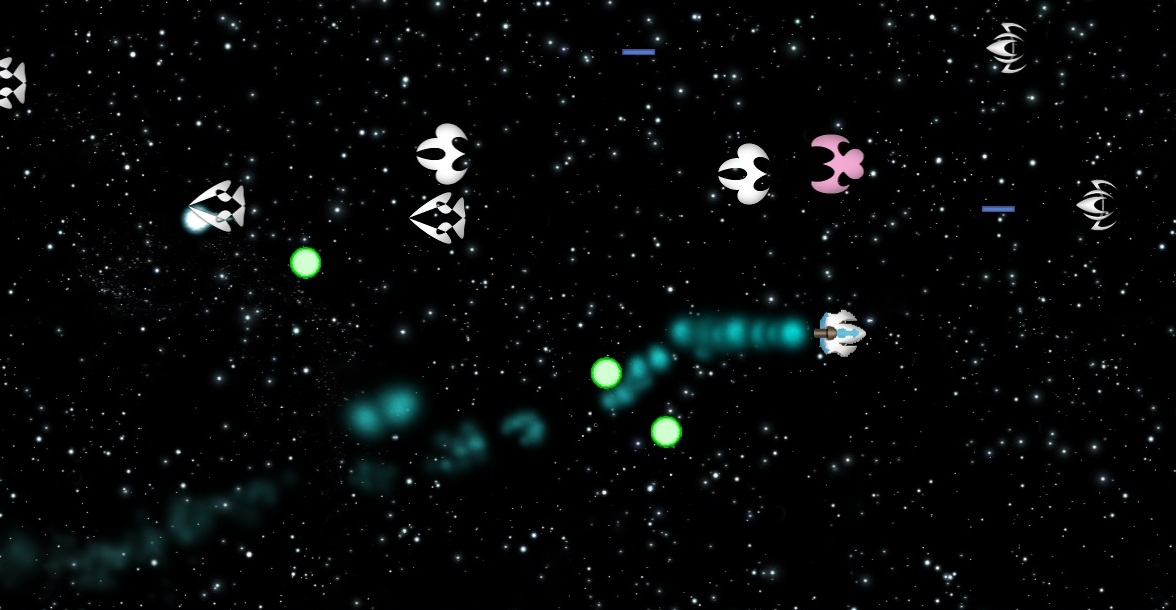
\includegraphics[width=13cm]{images/graphisme3.jpg}
	\vspace{1cm}
	\par 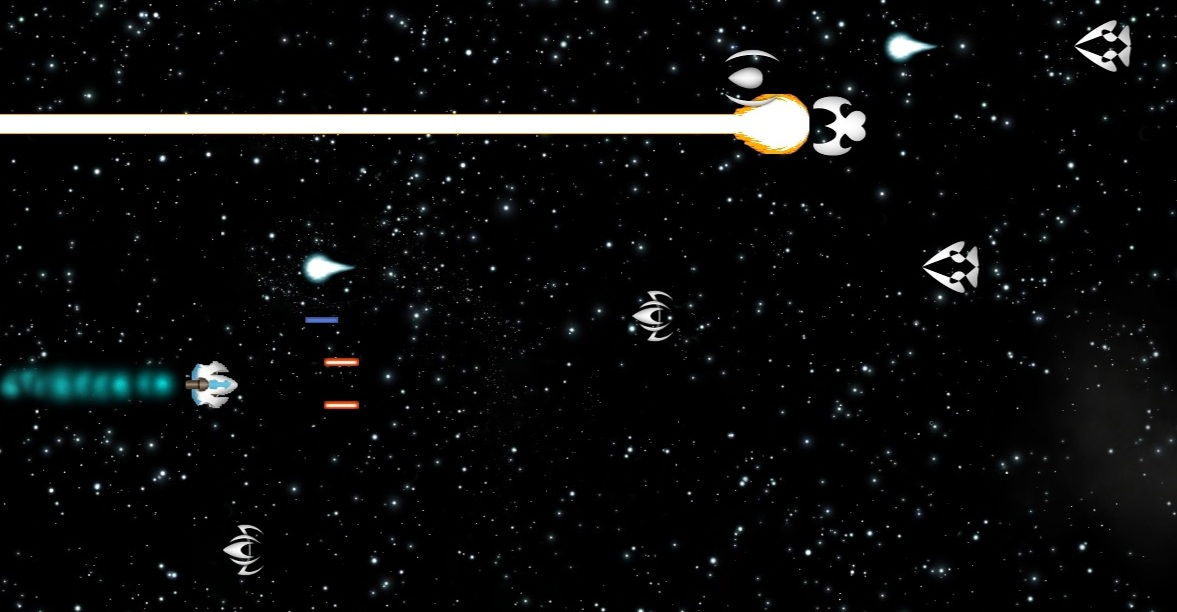
\includegraphics[width=13cm]{images/graphisme2.jpg}
\end{center}

\par Le menu et le logo ont demandé aussi beaucoup de travail, pour un résultat final de bonne qualité, que vous trouverez dans la partie Menu \& Score.

\subsubsection{Interface}
\par L'interface quant à elle, devait être intuitive et agréable à l'œil.
\par Au départ quasi-absente, elle est apparue dès la soutenance 2 sous une forme plus complète:

\begin{center}
	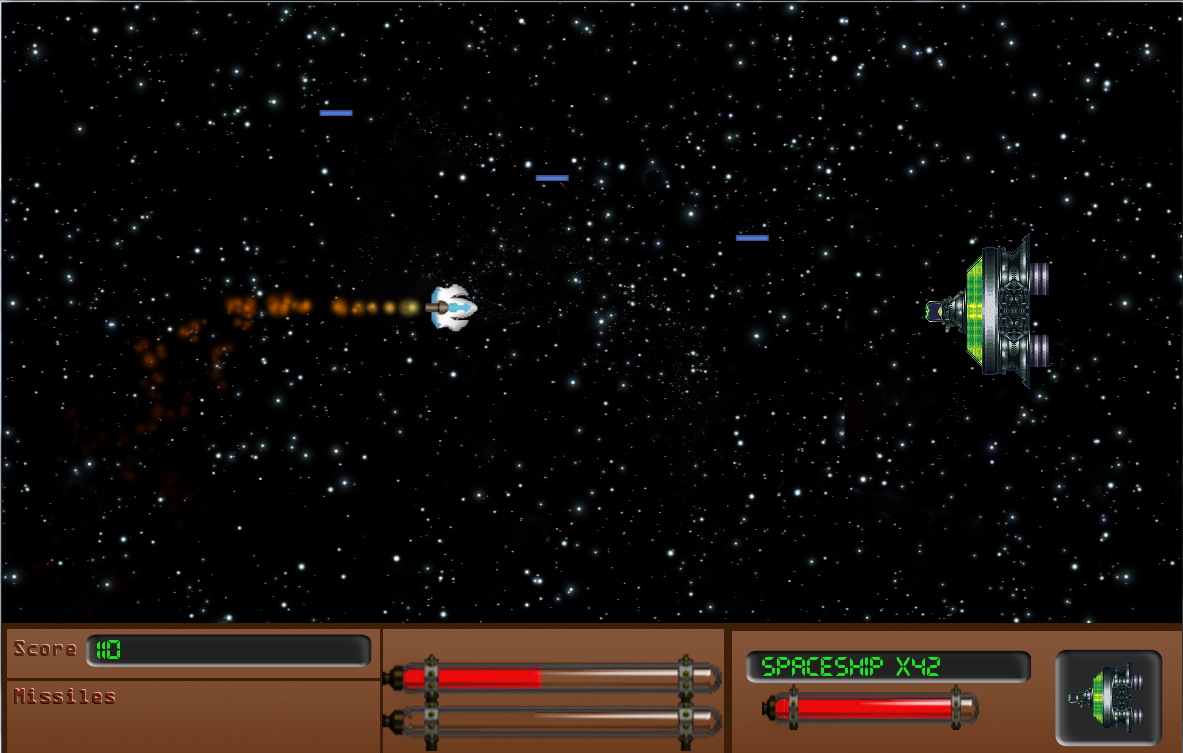
\includegraphics[width=13cm]{images/hud1.png}
\end{center}   
   
\par Vous pouvez y voir la vie du joueur, son score, et des informations sur le boss actuel. Toutefois, le plus dur rester à faire: Créer une interface intuitive. C'est pourquoi implémenter les missiles dans l'interface ne fut pas une tâche simple, et nous devions rendre cela beau graphiquement pour ne pas heurter l'œil du joueur.
\par Nous avons donc aussi décidé de rajouter une barre d'énergie dès la soutenance 3, permettant de tirer différents missiles disponibles dans l'arsenal du joueur. Au final, l'interface est simple, intuitive, et jolie graphiquement:

\begin{center}
	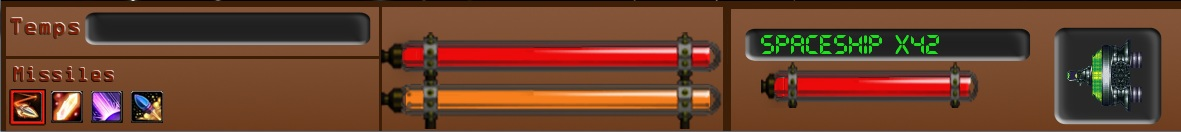
\includegraphics[width=15cm]{images/interface.jpg}
\end{center}

\subsubsection{Moteur à particules}
Le moteur a particules est d'une grande importance car il participe à l'immersion du joueur dans le jeu et les effets qu'il produit sont saisissants. Il est utilisé comme moteur de certains vaisseaux et certains missiles et dans les explosion.
Nous avons utilisé le moteur à particules MercuryEngine qui fournit une API pour permettre de changer le comportement des particules à la volée.
